\chapter{Optimizations of computer code}
\label{cha:optimizaiton}


\section{Vectorization}
\label{sec:optimizaiton_vectorization}

\section{Numba and code modifications}
\label{sec:optimizaiton_numba}
\subsection{Numba Library}
\label{ssec:numba_numba}
Numba is a Python compiler that transforms Python code to high performance machine code which supports NumPy arrays and functions and loops.
It could also work with CUDA to use Nvidia GPU.

\subsection{Implementation of $np.roll()$ in Numba}
\label{ssec:numba_nproll}
np.roll() was in fact implemented in Numba without support for axis argument.
However, this support is essential for our program. As the code is open source and the merge
commit of this feature can be viewed directly in GitHub, one simple work through is study
and copy those code and add the support for axis.

Let $A$ a matrix of dimension $n$, $B$ the matrix after shifting $shift$ along axis $axis$. 
Then we'll have for all $A[(x_i)_{i<n}], B[((x_i+(i==shift)*shift)\%shape[axis])_{i<n}]=A[(x_i)_{i<n}]$.

In order to prevent $if$ or $for$ overlap which consumes considerable amount of resources, a method using modulus operator is proposed.

Let $a=\prod^{n-axis}_{j=1}shape[n-j],b=\prod^{n-axis-1}_{j=1}shape[n-j]$. Apparently $b=a/shape[axis]$.

The code is not aware of the dimension of the matrix, so we'll have to operate through flatten array (of dimension 1).
A coordinate conversion formula is shown below.

If $A[(x_i)_{i<n}]=A.flat[idx], then idx=\sum^{n-1}_{i=0}x_i\prod^{n-i-1}_{j=1}shape[n-j]$.
So with $B[((x_i+(i==shift)*shift)\%shape[axis])_{i<n}]=A[(x_i)_{i<n}]$, we'll have : 
$$ idx_B=idx_A+((x_{axis}+shift)\%shape[axis]-x_{axis})\prod^{n-axis-1}_{j=1}shape[n-j]$$

Now we've only to get $x_{axis}$ from $idx_A$, firstly by $\%a$, we'll get $\sum^{axis}_{i=0}x_i\prod^{n-i-1}_{j=1}shape[n-j]$.

Then divide by $b$, take only the integer part we'll finally get $x_{axis}$.
The code of this process is shown in figure \ref{fig:nproll}.

\begin{figure}[!htb]
    \centering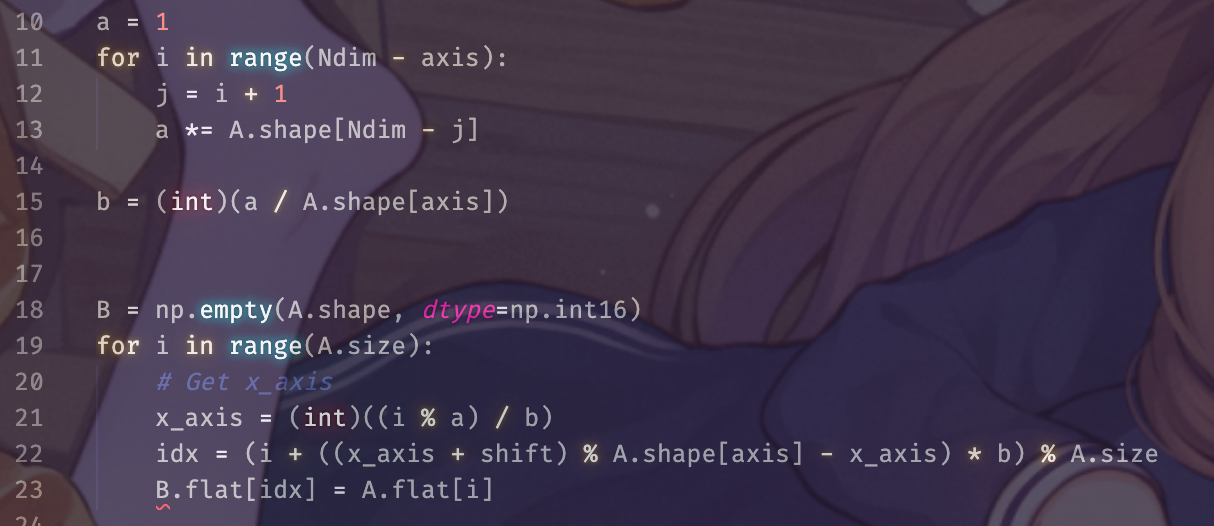
\includegraphics[width=0.6\linewidth]{Figs/implementationOfNpRoll.png}
    \caption{Code of $np.roll()$}
    \label{fig:nproll}
\end{figure}

However, the result of this optimization is not very satisfying. 
In some occasions, the implementation makes the program run slower than without Numba. 

\section{Pre-calculation of robot's coordinates (Project 2 only)}
\label{sec:optimizaiton_Precalculation}

Calculation of the robot's presence (spatial coordinates that the robot occupies) is rather resources expensive.
Since the robot's move in space could be regraded as translation, it could be pre-calculated.
Presences of the robot in different places could be obtained by simple addition of the presence of the robot of same arm configuration
and the difference in the coordinates of their origin point.
Let $ \mathcal{R} $ denote the set of points that are occupied by the robot at origin point $(0, 0)$.
Then the set of points occupied by the robot of same arm configurations at point $(x_0, y_0)$
will be $\{(x + x_0, y + y_0)|(x,y)\in\mathcal{R}\}$.
So at the beginning, we could directly calculate all the presences of the robot of all the arm configurations.
Then no more robot presence calculation is required.

For a neuronal space of size $ 192 \times 18 $,
without pre-calculation, generation of neuronal space takes about : 44.5 s.
With pre-calculation, generation of neuronal space takes about : 0.41 s, the preparation
of coordinates takes about 0.14 s.
An improvement of approximately $100\times$ can be expected from this method.
Greater the space, more significant will be the improvement.
Most importantly this method lowers the importance of the efficiency of the process of solving robot’s presence,
which is in addition, not a simple subject.